\begin{figure}[h] 
\centering 
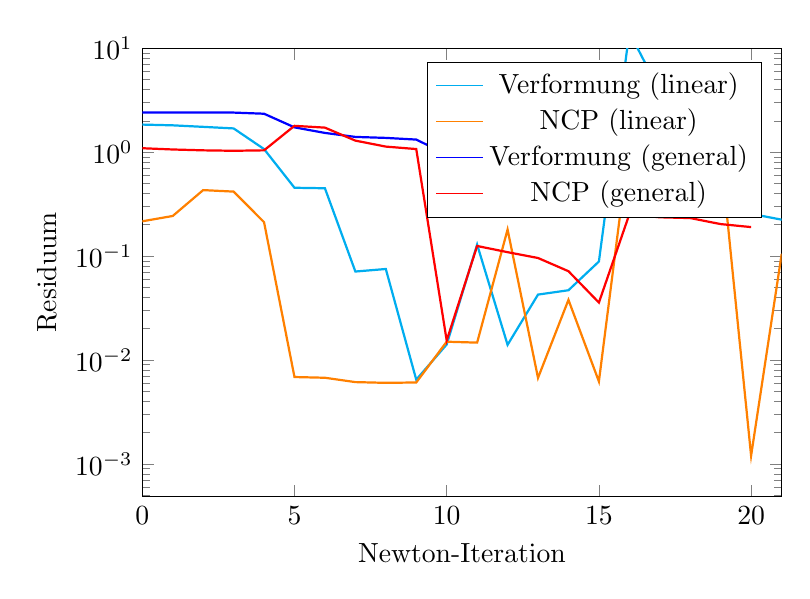
\begin{tikzpicture}[every plot/.append style={thick}] 
\begin{axis}[ 
label style={font=\normalsize}, 
xlabel={Newton-Iteration}, 
ylabel={Residuum}, 
xmin=0, xmax=21, 
ymode=log, 
ymin=0, ymax=10, 
width=0.8\textwidth, 
height=0.6\textwidth, 
legend pos=north east, 
legend style={cells={align=left}}, 
grid style=dashed, 
] 
\addplot[ 
color=cyan, 
] 
coordinates { 
(0, 1.84e+00)(1, 1.81e+00)(2, 1.75e+00)(3, 1.69e+00)(4, 1.07e+00)(5, 4.54e-01)(6, 4.49e-01)(7, 7.10e-02)(8, 7.51e-02)(9, 6.47e-03)(10, 1.41e-02)(11, 1.29e-01)(12, 1.40e-02)(13, 4.26e-02)(14, 4.69e-02)(15, 8.86e-02)(16, 1.42e+01)(17, 3.85e+00)(18, 8.75e-01)(19, 2.54e-01)(20, 2.55e-01)(21, 2.24e-01)(22, 1.96e-01)(23, 1.83e-01)(24, 2.51e-02)(25, 2.18e-03)(26, 3.89e-05)(27, 3.84e-05)(28, 5.50e-07)(29, 1.06e-05)(30, 1.66e-05)(31, 1.14e-05)(32, 6.36e-07)(33, 1.08e-05)(34, 1.66e-05)(35, 1.14e-05)(36, 6.36e-07)(37, 1.08e-05)(38, 1.66e-05)(39, 1.14e-05)(40, 6.36e-07)(41, 1.08e-05)(42, 1.66e-05)(43, 1.14e-05)(44, 6.36e-07)(45, 1.08e-05)(46, 1.66e-05)(47, 1.14e-05)(48, 6.36e-07)(49, 1.08e-05)(50, 1.66e-05)(51, 1.14e-05)(52, 6.36e-07)(53, 1.08e-05)(54, 1.66e-05)(55, 1.14e-05)(56, 6.36e-07)(57, 1.08e-05)(58, 1.66e-05)(59, 1.14e-05)(60, 6.36e-07)}; 
\addlegendentry{Verformung (linear)} 
\addplot[ 
color=orange, 
] 
coordinates { 
(0, 2.16e-01)(1, 2.43e-01)(2, 4.31e-01)(3, 4.17e-01)(4, 2.12e-01)(5, 6.86e-03)(6, 6.75e-03)(7, 6.13e-03)(8, 6.03e-03)(9, 6.08e-03)(10, 1.50e-02)(11, 1.47e-02)(12, 1.80e-01)(13, 6.73e-03)(14, 3.79e-02)(15, 6.22e-03)(16, 1.25e+00)(17, 1.38e+00)(18, 8.08e-01)(19, 9.89e-01)(20, 1.20e-03)(21, 1.03e-01)(22, 1.45e-01)(23, 7.26e-02)(24, 8.74e-04)(25, 8.79e-04)(26, 8.77e-04)(27, 8.64e-04)(28, 8.77e-04)(29, 8.71e-04)(30, 8.77e-04)(31, 8.63e-04)(32, 8.77e-04)(33, 8.71e-04)(34, 8.77e-04)(35, 8.63e-04)(36, 8.77e-04)(37, 8.71e-04)(38, 8.77e-04)(39, 8.63e-04)(40, 8.77e-04)(41, 8.71e-04)(42, 8.77e-04)(43, 8.63e-04)(44, 8.77e-04)(45, 8.71e-04)(46, 8.77e-04)(47, 8.63e-04)(48, 8.77e-04)(49, 8.71e-04)(50, 8.77e-04)(51, 8.63e-04)(52, 8.77e-04)(53, 8.71e-04)(54, 8.77e-04)(55, 8.63e-04)(56, 8.77e-04)(57, 8.71e-04)(58, 8.77e-04)(59, 8.63e-04)(60, 8.77e-04)}; 
\addlegendentry{NCP (linear)} 
\addplot[ 
color=blue, 
] 
coordinates { 
(0, 2.41e+00)(1, 2.40e+00)(2, 2.40e+00)(3, 2.40e+00)(4, 2.34e+00)(5, 1.73e+00)(6, 1.53e+00)(7, 1.40e+00)(8, 1.37e+00)(9, 1.32e+00)(10, 9.49e-01)(11, 9.41e-01)(12, 9.01e-01)(13, 8.79e-01)(14, 7.99e-01)(15, 5.85e-01)(16, 4.76e-01)(17, 4.74e-01)(18, 4.99e-01)(19, 5.13e-01)(20, 5.18e-01)}; 
\addlegendentry{Verformung (general)} 
\addplot[ 
color=red, 
] 
coordinates { 
(0, 1.09e+00)(1, 1.06e+00)(2, 1.04e+00)(3, 1.03e+00)(4, 1.04e+00)(5, 1.79e+00)(6, 1.72e+00)(7, 1.29e+00)(8, 1.13e+00)(9, 1.07e+00)(10, 1.54e-02)(11, 1.25e-01)(12, 1.09e-01)(13, 9.58e-02)(14, 7.15e-02)(15, 3.57e-02)(16, 2.52e-01)(17, 2.36e-01)(18, 2.32e-01)(19, 2.03e-01)(20, 1.90e-01)}; 
\addlegendentry{NCP (general)} 
\end{axis} 
\end{tikzpicture} 
\caption{Residuen des Stoffgesetzes 'St.Venant' mit Hinderniss 'Hut' und 578 Freiheitsgraden für die Verschiebung.} 
\label{fiq:St.Venant_Hut_level3} 
\end{figure} 
